\documentclass[aspectratio=169]{beamer}

%% ---------------------------------------------------------------------------
%%  Extracting Blame — talk slides  (target: 20–25 min + Q&A)
%%  Theme: Metropolis (mtheme). Build: make slides  (LuaLaTeX; do NOT use
%%  XeLaTeX — it leaks overlay transparency across the pgfpages notes layout,
%%  making base-layer slide text nearly invisible)
%%
%%  SPEAKER NOTES / SCRIPT
%%    The numbered main deck is scripted for roughly 23 minutes. Every main
%%    frame has a complete spoken script and a time budget; the backup frames
%%    after the thank-you slide are for Q&A. <click> markers in the script sit
%%    where the next overlay is revealed.
%%
%%    DEFAULT BUILD: notes on the right half of a double-width page
%%    (show notes on second screen=right) — rehearsal-ready out of the box.
%%    For the clean presentation PDF: comment out that \setbeameroption line.
%%    For a notes-only handout: use \setbeameroption{show only notes} instead.
%%
%%  Color system:
%%    srcBlue   — source language (CoC)
%%    tgtTeal   — target language (Fω + blame)
%%    dynOrange — dynamic boundary
%%    blameRed  — blame, failure, alerts
%%    okGreen   — mechanized facts
%% ---------------------------------------------------------------------------

\usetheme[progressbar=frametitle]{metropolis}
\metroset{block=fill, numbering=fraction, sectionpage=none}

\usepackage{amssymb}
\usepackage{mathpartir}
\usepackage{listings}
\usepackage{booktabs}
\usepackage{xcolor}
\usepackage{pgfpages}
\usepackage{fontawesome5}
\usetikzlibrary{arrows.meta,positioning,calc,fit,shapes.geometric}

%% --- speaker notes (default ON; comment out for the clean deck) -------------
\setbeameroption{show notes on second screen=right}
% \setbeameroption{show only notes}
\setbeamertemplate{note page}[plain]
\setbeamerfont{note page}{size=\footnotesize}

%% --- palette ----------------------------------------------------------------
\definecolor{srcBlue}{HTML}{2A6099}
\definecolor{tgtTeal}{HTML}{0F766E}
\definecolor{dynOrange}{HTML}{C2410C}
\definecolor{blameRed}{HTML}{B91C1C}
\definecolor{okGreen}{HTML}{15803D}
\definecolor{outBg}{HTML}{F4F1EA}
\definecolor{accentOrange}{HTML}{EB811B}

\setbeamercolor{progress bar}{fg=accentOrange}
\setbeamercolor{alerted text}{fg=blameRed}
\setbeamercolor{example text}{fg=okGreen}
\setbeamercolor{block title}{fg=black,bg=black!13}
\setbeamercolor{block body}{fg=black,bg=black!5}
\setbeamercolor{block title alerted}{fg=white,bg=blameRed}
\setbeamercolor{block body alerted}{fg=black,bg=blameRed!7}
\setbeamercolor{block title example}{fg=white,bg=okGreen}
\setbeamercolor{block body example}{fg=black,bg=okGreen!7}

%% --- reusable visual language ------------------------------------------------
\setbeamercolor{source card}{fg=black,bg=srcBlue!9}
\setbeamercolor{target card}{fg=black,bg=tgtTeal!9}
\setbeamercolor{dynamic card}{fg=black,bg=dynOrange!10}
\setbeamercolor{danger card}{fg=black,bg=blameRed!9}
\setbeamercolor{success card}{fg=black,bg=okGreen!9}
\setbeamercolor{neutral card}{fg=black,bg=black!6}
\setbeamercolor{terminal card}{fg=white,bg=black!86}

\newenvironment{sourcecard}[1]{%
  \begin{beamercolorbox}[wd=\linewidth,sep=0.62em,rounded=true]{source card}%
  {\color{srcBlue}\bfseries #1}\par\smallskip
}{\end{beamercolorbox}}
\newenvironment{targetcard}[1]{%
  \begin{beamercolorbox}[wd=\linewidth,sep=0.62em,rounded=true]{target card}%
  {\color{tgtTeal}\bfseries #1}\par\smallskip
}{\end{beamercolorbox}}
\newenvironment{dynamiccard}[1]{%
  \begin{beamercolorbox}[wd=\linewidth,sep=0.62em,rounded=true]{dynamic card}%
  {\color{dynOrange}\bfseries #1}\par\smallskip
}{\end{beamercolorbox}}
\newenvironment{dangercard}[1]{%
  \begin{beamercolorbox}[wd=\linewidth,sep=0.62em,rounded=true]{danger card}%
  {\color{blameRed}\bfseries #1}\par\smallskip
}{\end{beamercolorbox}}
\newenvironment{successcard}[1]{%
  \begin{beamercolorbox}[wd=\linewidth,sep=0.62em,rounded=true]{success card}%
  {\color{okGreen}\bfseries #1}\par\smallskip
}{\end{beamercolorbox}}
\newenvironment{neutralcard}[1]{%
  \begin{beamercolorbox}[wd=\linewidth,sep=0.62em,rounded=true]{neutral card}%
  {\color{black!75}\bfseries #1}\par\smallskip
}{\end{beamercolorbox}}

\newcommand{\talkpill}[2]{%
  \tikz[baseline=(pill.base)]
    \node[rounded corners=2.2pt,fill=#1!12,text=#1!85!black,
      inner xsep=0.58em,inner ysep=0.25em] (pill) {\strut #2};}

\tikzset{
  flow arrow/.style={-{Latex[length=2.5mm]},draw=black!48,line width=1.05pt},
  source node/.style={rounded corners=3pt,draw=srcBlue!45,fill=srcBlue!7,
    line width=0.6pt,inner sep=7pt,align=center},
  target node/.style={rounded corners=3pt,draw=tgtTeal!48,fill=tgtTeal!7,
    line width=0.6pt,inner sep=7pt,align=center},
  dynamic node/.style={rounded corners=3pt,draw=dynOrange!55,fill=dynOrange!8,
    line width=0.6pt,inner sep=7pt,align=center},
  danger node/.style={rounded corners=3pt,draw=blameRed!55,fill=blameRed!7,
    line width=0.6pt,inner sep=7pt,align=center},
  success node/.style={rounded corners=3pt,draw=okGreen!52,fill=okGreen!7,
    line width=0.6pt,inner sep=7pt,align=center},
  neutral node/.style={rounded corners=3pt,draw=black!22,fill=black!5,
    line width=0.6pt,inner sep=7pt,align=center}
}

%% --- notation macros --------------------------------------------------------
\newcommand{\dyn}{{\color{dynOrange}\mathsf{Dyn}}}
\newcommand{\kstar}{\ensuremath{\star}}
\newcommand{\karr}{\ensuremath{\Rightarrow}}
\newcommand{\PropS}{\mathsf{Prop}}
\newcommand{\SetS}{\mathsf{Set}}
\newcommand{\KindS}{\mathsf{Kind}}
\newcommand{\Nat}{\mathsf{Nat}}
\newcommand{\castt}[4]{{\color{tgtTeal}\langle} #2 {\color{tgtTeal}\Rightarrow}
  #3 {\color{tgtTeal}\rangle^{#4}}\,#1}
\newcommand{\gnd}[2]{\mathsf{gnd}(#1, #2)}
\newcommand{\isgnd}[2]{\mathsf{is\_gnd}(#1, #2)}
\newcommand{\blame}[1]{{\color{blameRed}\mathsf{blame}\,#1}}
\newcommand{\nub}[4]{\nu #1{:}#2 := #3.\,#4}
\newcommand{\ext}{\mathcal{E}}
\newcommand{\extt}{\mathcal{T}}
\newcommand{\extk}{\mathcal{K}}
\newcommand{\extc}{\mathcal{C}}
\newcommand{\coerce}[3]{\mathsf{coerce}\,#1\,#2\,#3}
\newcommand{\islarge}{\mathsf{large}}
\newcommand{\nf}{\mathsf{nf}}
\newcommand{\lint}{\ell_{\mathsf{int}}}
\newcommand{\reduces}{\longrightarrow}
\newcommand{\reducesstar}{\longrightarrow^{*}}
\newcommand{\sepsim}{\mathrel{\lesssim}}
\newcommand{\hastype}[3]{#1 \vdash #2 : #3}
\newcommand{\src}[1]{\textcolor{srcBlue}{#1}}
\newcommand{\tgt}[1]{\textcolor{tgtTeal}{#1}}
\newcommand{\mech}[1]{\textcolor{okGreen}{\texttt{#1}}}
\newcommand{\click}{{\color{accentOrange}\textbf{\textless click\textgreater}}~}

%% --- listings: CoC source vs. REPL output -----------------------------------
\lstdefinelanguage{coc}{
  morekeywords={fun,forall,Set,Prop,Kind,Axiom,Definition,Infer,Check,Extract,let,in},
  sensitive=true,
  morecomment=[s]{(*}{*)}
}
\lstset{
  language=coc,
  basicstyle=\ttfamily\footnotesize,
  keywordstyle=\color{srcBlue}\bfseries,
  commentstyle=\color{gray}\itshape,
  columns=fullflexible,
  keepspaces=true,
  showstringspaces=false,
  breaklines=false,
  xleftmargin=1em
}
\lstdefinestyle{replout}{
  language={},
  basicstyle=\ttfamily\footnotesize\color{tgtTeal!90!black},
  backgroundcolor=\color{outBg},
  frame=leftline, framerule=2pt, rulecolor=\color{accentOrange},
  framesep=6pt, xleftmargin=1.5em,
  keywords={Dyn}, keywordstyle=\color{dynOrange}\bfseries,
  morekeywords=[2]{blame}, keywordstyle={[2]\color{blameRed}\bfseries},
  morekeywords=[3]{cast}, keywordstyle={[3]\color{tgtTeal}\bfseries},
  columns=fullflexible, keepspaces=true, breaklines=false
}

\title{Extracting Blame}
\subtitle{Keeping Dependent Guarantees Across the Extraction Boundary}
\author{Joomy Korkut}
\institute{Bloomberg\\[1.2ex]
  {\scriptsize
   {\color{accentOrange}\faEnvelope}\hspace{0.5em}%
   {\color{black!65}\texttt{jkorkut@bloomberg.net}}%
   \hspace{1.6em}%
   {\color{accentOrange}\faTwitter}\hspace{0.5em}%
   {\color{black!65}\texttt{@joomy}}%
   \hspace{1.6em}%
   {\color{accentOrange}\faMastodon}\hspace{0.5em}%
   {\color{black!65}\texttt{@joomy@functional.cafe}}}}
\date{}

\begin{document}

\begin{frame}[plain]
  \begin{tikzpicture}[remember picture,overlay]
    \fill[srcBlue!8]
      (current page.north west) rectangle
      ([xshift=0.13cm]current page.south west);
    \fill[accentOrange]
      ([xshift=0.13cm]current page.north west) rectangle
      ([xshift=0.20cm]current page.south west);
    \fill[tgtTeal!4]
      ([xshift=-4.55cm]current page.north east) rectangle
      (current page.south east);
  \end{tikzpicture}

  \begin{columns}[c,onlytextwidth]
    \column{0.60\textwidth}
    {\color{black!82}\fontsize{25}{29}\selectfont\bfseries
      Extracting Blame\par}
    \vspace{0.65em}
    {\color{black!72}\large
      Keeping Dependent Guarantees\\[-0.15ex]
      Across the Extraction Boundary\par}

    \vspace{0.9em}
    {\color{accentOrange}\rule{\linewidth}{1.05pt}}
    \vspace{1.15em}

    {\large Joomy Korkut}\par
    \smallskip
    {\color{black!65}Bloomberg}\par
    \medskip
    {\scriptsize
      {\color{accentOrange}\faEnvelope}\hspace{0.45em}%
      {\color{black!65}\texttt{jkorkut@bloomberg.net}}\\[0.45ex]
      {\color{accentOrange}\faTwitter}\hspace{0.45em}%
      {\color{black!65}\texttt{@joomy}}%
      \hspace{1.4em}%
      {\color{accentOrange}\faMastodon}\hspace{0.45em}%
      {\color{black!65}\texttt{@joomy@functional.cafe}}}

    \column{0.34\textwidth}
    \centering
    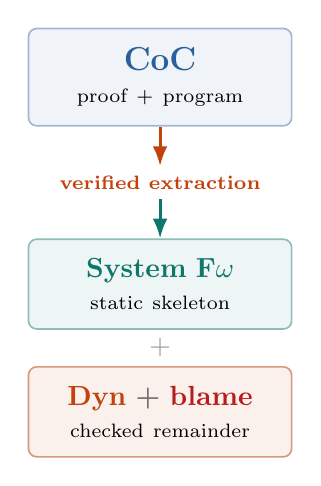
\begin{tikzpicture}[node distance=0.58cm]
      \node[source node,text width=2.85cm] (coc) {%
        {\color{srcBlue}\bfseries\large CoC}\\[-0.1ex]
        \scriptsize proof + program};
      \node[below=0.5cm of coc,font=\scriptsize\bfseries,
        text=dynOrange] (boundary) {verified extraction};
      \node[target node,text width=2.85cm,below=0.5cm of boundary] (static) {%
        {\color{tgtTeal}\bfseries System F$\omega$}\\[-0.1ex]
        \scriptsize static skeleton};
      \node[dynamic node,text width=2.85cm,below=0.46cm of static] (dynamic) {%
        {\color{dynOrange}\bfseries Dyn}
        {\color{black!55}\bfseries +}
        {\color{blameRed}\bfseries blame}\\[-0.1ex]
        \scriptsize checked remainder};
      \draw[flow arrow,draw=dynOrange] (coc) -- (boundary);
      \draw[flow arrow,draw=tgtTeal] (boundary) -- (static);
      \node[text=black!42,font=\bfseries] at
        ($(static.south)!0.5!(dynamic.north)$) {$+$};
    \end{tikzpicture}
  \end{columns}
  \note{%
    \textbf{[0:00 — 0:30]}\\
    Hi everyone! I'm Joomy. This talk starts with a small refactoring that
    Rocq's type system rejects, but the extracted OCaml program accepts --- and
    then segfaults. That example exposes a boundary we do not talk about enough:
    when verified code leaves a proof assistant, which guarantees survive in
    the target language? I will show a verified translation that keeps the
    static structure its target can express and turns the genuine remainder
    into an explicit, checked failure instead of an unchecked cast.
  }
\end{frame}

%% ==========================================================================
\section{The problem}
%% ==========================================================================

\begin{frame}{A format value can determine a function's type}
  \begin{center}
  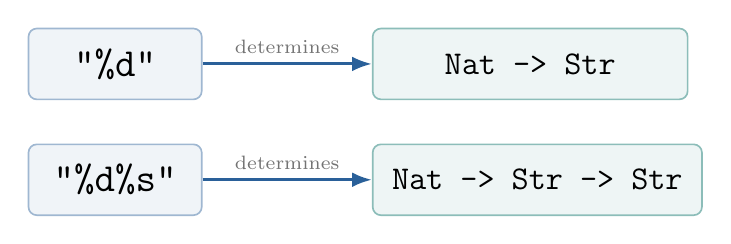
\begin{tikzpicture}[node distance=0.55cm and 2.15cm]
    \node[source node,minimum width=2.2cm,minimum height=0.9cm]
      (fmt1) {{\Large\texttt{"\%d"}}};
    \node[target node,right=of fmt1,minimum width=4.0cm,minimum height=0.9cm]
      (typ1) {{\large\texttt{Nat -> Str}}};
    \node[source node,below=of fmt1,minimum width=2.2cm,minimum height=0.9cm]
      (fmt2) {{\Large\texttt{"\%d\%s"}}};
    \node[target node,right=of fmt2,minimum width=4.0cm,minimum height=0.9cm]
      (typ2) {{\large\texttt{Nat -> Str -> Str}}};
    \draw[flow arrow,srcBlue] (fmt1) -- node[above,black!55,font=\scriptsize]
      {determines} (typ1);
    \draw[flow arrow,srcBlue] (fmt2) -- node[above,black!55,font=\scriptsize]
      {determines} (typ2);
  \end{tikzpicture}
  \end{center}

  \pause
  \medskip
  \begin{sourcecard}{\faProjectDiagram\quad The dependent-type idea}
    A \emph{value} --- the format --- determines the \emph{type} of the
    function that interprets it.
  \end{sourcecard}
  \note{%
    \textbf{[0:30 — 1:30]}\\
    Here is the only dependent-type idea you need for this talk. The format
    percent-d describes a function that consumes a natural number and returns a
    string. Percent-d percent-s describes a function with two arguments. The
    format is ordinary data, but it determines the function's type.\\
    \click That is what ``dependent'' means in this example: a value appears in,
    or computes, a type. The source type checker can therefore keep the format
    and every call site synchronized. You do not need to know the Calculus of
    Constructions to follow the rest; keep this one relationship in mind.
  }
\end{frame}

\begin{frame}[fragile]{Rocq catches the drift}
  \begin{columns}[T,onlytextwidth]
    \column{0.43\textwidth}
    \begin{sourcecard}{\texttt{Fmt A} carries the promise}
      \small\ttfamily
      sprintf : Fmt A -> A\\[0.55ex]
      fint : Fmt A ->\\
      \hspace*{2.2em}Fmt (Nat -> A)\\[0.55ex]
      fstr : Fmt A ->\\
      \hspace*{2.2em}Fmt (Str -> A)
    \end{sourcecard}

    \column{0.53\textwidth}
    \pause
    \begin{successcard}{\faCheckCircle\quad One argument / accepted}
      \small\ttfamily
      Check sprintf\\
      \quad (Nat -> Str)\\
      \quad (fint Str fstop).
    \end{successcard}

    \smallskip
    \begin{dangercard}{\faTimesCircle\quad Two arguments / rejected}
      \small\ttfamily
      Check sprintf\\
      \quad (Nat -> Str -> Str)\\
      \quad (fint Str fstop).
    \end{dangercard}
  \end{columns}
  \note{%
    \textbf{[1:30 — 2:30]}\\
    Here is the small amount of source notation behind it. A value of type
    \texttt{Fmt A} is a format denoting an \texttt{A}. Adding percent-d changes
    the index from \texttt{A} to \texttt{Nat to A}; percent-s does the same for
    strings. So \texttt{sprintf} can return exactly the function described by
    its format.\\
    \click The first check says that a one-percent-d format denotes a
    one-argument function. Rocq accepts it. The second call claims the same
    format takes two arguments. Rocq rejects it. This is not a theorem about a
    distant specification: it is an everyday interface guarantee enforced at
    the call site.
  }
\end{frame}

\begin{frame}[fragile]{Stock extraction severs the link}
  \begin{columns}[T,onlytextwidth]
    \column{0.40\textwidth}
    \begin{sourcecard}{What the source promised}
      \begin{center}
        \Large\src{\texttt{Fmt A $\to$ A}}
      \end{center}
      \smallskip
      The \emph{format} determines \texttt{A}.
    \end{sourcecard}

    \column{0.56\textwidth}
    \pause
    \begin{dangercard}{What OCaml receives}
      \small\ttfamily
      type 'x fmt =\\
      \quad Fstop | Flit of str * 'x fmt\\
      \quad | Fint of \_\_ fmt\\
      \quad | Fstr of \_\_ fmt\\[0.7ex]
      val sprintf : 'a fmt -> 'a
    \end{dangercard}
  \end{columns}

  \medskip
  \begin{center}
    \talkpill{blameRed}{the caller chooses \texttt{'a}}
    \hspace{0.6em}
    \talkpill{blameRed}{\texttt{Obj.magic} promises it was right}
  \end{center}
  \note{%
    \textbf{[2:30 — 3:40]}\\
    Now we extract that program with Rocq 9.0's stock OCaml extraction.\\
    \click The result is still typed OCaml, but read what the type says.
    \texttt{Fint} can take a format at one type and return a format at any other
    type. And \texttt{sprintf} says: give me a format and I can return whatever
    type the caller asks for. The format no longer determines the function; the
    caller does. To implement that impossible promise, the extracted body uses
    \texttt{Obj.magic}, OCaml's unchecked cast. The source program remains
    verified inside Rocq. What broke is its ability to compose safely through
    the exported target interface.
  }
\end{frame}

\begin{frame}[fragile]{A plausible refactoring, a segfault}
  \begin{columns}[T,onlytextwidth]
    \column{0.57\textwidth}
    \begin{neutralcard}{The refactoring drift}
      \small\ttfamily
      (* format: "\%d"; caller: "\%d\%s" *)\\[0.5ex]
      let report : nat -> str -> str =\\
      \quad sprintf (Fint Fstop)\\[0.5ex]
      let \_ = report O Sempty
    \end{neutralcard}

    \column{0.39\textwidth}
    \onslide<2->{%
    \begin{dangercard}{\faExclamationTriangle\quad Runtime outcome}
      \begin{center}
        \LARGE\alert{SIGSEGV}

        \smallskip
        \small Not an exception.\\
        Not catchable.\\
        Names nobody.
      \end{center}
    \end{dangercard}}
  \end{columns}

  \onslide<3->{%
  \smallskip
  \begin{beamercolorbox}[wd=\linewidth,sep=0.72em,rounded=true]{danger card}
    \begin{columns}[c,onlytextwidth]
      \column{0.18\textwidth}
      \centering\color{blameRed}\fontsize{24}{25}\selectfont\bfseries 7/18
      \column{0.78\textwidth}
      \small Stock-extracted example idioms use \texttt{Obj.magic} or
      \texttt{Obj.t}. This is a boundary problem, not a toy corner case.
    \end{columns}
  \end{beamercolorbox}}
  \note{%
    \textbf{[3:40 — 4:50]}\\
    So someone changes a format in one place but misses one call site --- the
    exact refactoring error type-safe printf exists to prevent. OCaml accepts
    this because the weakened interface lets the one-argument closure pose as a
    two-argument function.\\
    \click The second application tries to call a data block as a closure and
    the process receives SIGSEGV. No OCaml exception is raised, so the failure
    cannot be caught, and no boundary is identified.\\
    \click This is not unique to printf. Seven of the eighteen dependent
    programming idioms in our artifact need unchecked casts or \texttt{Obj.t}
    interfaces under stock Rocq extraction: bounds-checked indexing,
    heterogeneous data, typed interpreters, and others. If proofs are going to
    protect deployed code, the handoff to the surrounding ecosystem matters.
  }
\end{frame}

\begin{frame}{What should extraction promise?}
  \begin{columns}[T,onlytextwidth]
    \column{0.31\textwidth}
    \begin{successcard}{\faCheckCircle\quad Best case}
      Preserve enough structure to reject the mistake
      \textcolor{okGreen}{statically}.
    \end{successcard}

    \column{0.31\textwidth}
    \onslide<2->{\begin{dynamiccard}{\faLock\quad Fallback}
      Cross a checked boundary whose failure is explicit
      \textcolor{blameRed}{blame}.
    \end{dynamiccard}}

    \column{0.31\textwidth}
    \onslide<3->{\begin{dangercard}{\faTimesCircle\quad Never}
      Hide the gap behind an unchecked cast and undefined behavior.
    \end{dangercard}}
  \end{columns}

  \onslide<4->{%
  \bigskip
  \begin{alertblock}{The question}
    How much dependent structure can a richer typed target preserve?\\[-0.2ex]
    Can we verify both the translation and its fallback?
  \end{alertblock}}
  \note{%
    \textbf{[4:50 — 5:50]}\\
    This gives us a hierarchy of outcomes. First, the best outcome is not a
    runtime check at all. If the target can express the relationship, keep it
    static and reject the mistake before the program runs.\\
    \click If the target genuinely cannot express the dependency, use a typed,
    checked boundary. A mismatch then becomes explicit blame: an ordinary result
    in the target semantics, carrying a label.\\
    \click What we must not do is pretend the types agree and delegate the
    consequences to undefined behavior.\\
    \click So our question is: how much can we preserve, where exactly must we
    fall back, and can Rocq check the answer? This separation is important:
    printf will stay static; blame is for the harder residue.
  }
\end{frame}

%% ==========================================================================
\section{The design}
%% ==========================================================================

\begin{frame}{One translation, three outcomes}
  \begin{columns}[T,onlytextwidth]
    \column{0.31\textwidth}
    \begin{targetcard}{\faLayerGroup\quad 1 / Preserve}
      Type structure the target can express.

      \smallskip
      \src{\texttt{Fmt A}} $\rightsquigarrow$ \tgt{\texttt{Fmt A}}
    \end{targetcard}

    \column{0.31\textwidth}
    \begin{neutralcard}{\faCode\quad 2 / Erase}
      Term indices from target types.

      \smallskip
      \src{\texttt{Vec A n}} $\rightsquigarrow$ \tgt{\texttt{Vec A}}
    \end{neutralcard}

    \column{0.31\textwidth}
    \begin{dynamiccard}{\faRandom\quad 3 / Dynamize}
      Values used where the target needs a type.

      \smallskip
      \src{\texttt{El c}} $\rightsquigarrow$
      \mbox{$\dyn + \blame{\mathsf{int}}$}
    \end{dynamiccard}
  \end{columns}

  \pause
  \bigskip
  \begin{center}
    \talkpill{tgtTeal}{Preserve what can stay static}
    \hspace{0.6em}
    \talkpill{dynOrange}{Expose the remainder explicitly}
  \end{center}
  \note{%
    \textbf{[5:50 — 6:50]}\\
    Our translation has one policy and three outcomes. On the left, preserve:
    polymorphism, functions over types, and higher-kinded type families remain
    genuine target type structure. In the middle, erase: a vector's length may
    disappear from its target type even if the length remains as runtime data.
    On the right, dynamize: when an ordinary value is being used as a type and
    the target has no such type-level object, that residue goes through Dyn and
    a reserved internal blame marker.\\
    \click We call the translation optimistic because it does not defensively
    make everything dynamic. It preserves every part this translation knows how
    to express statically and reaches for Dyn only at the genuine boundary.
  }
\end{frame}

\begin{frame}{The type-theoretic gap, precisely}
  \begin{columns}[T,onlytextwidth]
    \column{0.43\textwidth}
    \begin{sourcecard}{CoC / the source}
      \begin{center}\Large$\Pi(x{:}A).\,B\,x$\end{center}
      \small Unified terms and types. The codomain $B\,x$ may mention the
      \emph{term} $x$.
    \end{sourcecard}

    \column{0.08\textwidth}
    \onslide<2->{\vspace{1.3cm}\centering
      {\color{accentOrange}\Large\faArrowRight}}

    \column{0.43\textwidth}
    \onslide<2->{\begin{targetcard}{System F$\omega$ / the static core}
      \begin{center}
        A \to B
        \quad
        \forall \alpha{:}K.\,A
        \quad
        \Lambda\alpha{:}K.\,A
      \end{center}
      \small Higher-kinded type functions --- but no \emph{term value} $x$
      inside a type.
    \end{targetcard}}
  \end{columns}

  \onslide<3->{%
  \smallskip
  \begin{dynamiccard}{\faBalanceScale\quad The middle ground}
    \centering\small F$\omega$ is richer than ML, less dependent than CoC.\\[-0.2ex]
    Preserve its static skeleton; erase or dynamize the remaining term dependency.
  \end{dynamiccard}}
  \note{%
    \textbf{[6:50 — 8:00]}\\
    Let me name the type-theoretic gap more precisely. Our source is the Calculus
    of Constructions, the small dependent core behind Rocq. Its central type is
    the dependent product, Pi x of A, B x. Ordinary functions and universal
    quantification are both instances of it, and the result type may mention the
    value x. CoC also treats terms and types in one uniform syntax.\\
    \click The static core of our target is System F-omega. This is substantially
    richer than ML polymorphism: it has explicit type abstraction and
    application, type-level lambda functions, and higher kinds. That is why it
    can preserve structures like Fmt and computed type-level codes. But it still
    separates terms from types, so an ordinary term value cannot occur in a
    target type.\\
    \click That makes F-omega a useful middle ground. Paulin-Mohring already
    connected CoC and F-omega in 1989. We keep that expressive static skeleton
    and add Dyn and blame for the part of dependency that crosses the remaining
    term-to-type boundary.
  }
\end{frame}

\begin{frame}{Preserve: \texttt{sprintf} stays static}
  \begin{center}
  \begin{tikzpicture}[node distance=0.7cm and 1.30cm]
    \node[source node,minimum width=1.9cm] (fmt)
      {{\large\texttt{"\%d"}}};
    \node[source node,right=of fmt,minimum width=3.25cm] (srct)
      {\texttt{Fmt (Nat -> Str)}};
    \draw[flow arrow,srcBlue] (fmt) -- node[above,black!55,font=\scriptsize]
      {indexes} (srct);

    \onslide<2->{%
      \node[target node,right=of srct,minimum width=2.55cm]
        (tgt) {{\large\texttt{Nat -> Str}}};
      \draw[flow arrow,tgtTeal] (srct) -- node[above,black!55,font=\scriptsize]
        {extract} (tgt);
      \node[danger node,below=of srct,text width=3.2cm]
        (claim) {\small client claims\\\texttt{Nat -> Str -> Str}};
      \node[danger node,right=of claim,minimum width=2.55cm,font=\bfseries]
        (reject) {\faTimesCircle\quad TYPE ERROR};
      \draw[flow arrow,blameRed] (claim) -- (reject);
    }
  \end{tikzpicture}
  \end{center}

  \onslide<2->{%
  \begin{center}
    \talkpill{okGreen}{0 Dyn}
    \hspace{0.35em}\talkpill{okGreen}{0 casts}
    \hspace{0.35em}\talkpill{okGreen}{0 blame}
    \hspace{0.7em}\small The arity is ordinary F$\omega$ structure.
  \end{center}}
  \note{%
    \textbf{[8:00 — 9:00]}\\
    Now return to printf. The percent-d format has source type
    \texttt{Fmt of Nat to Str}.\\
    \click Under our translation, the extracted application has target type
    \texttt{Nat to Str}. This is a statement about the translated target type,
    justified by the well-typedness theorem; the REPL's \texttt{Check} command
    itself checks the source term. F-omega can express the computed arrow type,
    so the drifted two-argument client is a
    target type error again, before evaluation. The richer target preserves the
    useful static guarantee that stock ML extraction lost.
  }
\end{frame}

\begin{frame}{Erase: indices leave the type, not the program}
  \begin{columns}[c,onlytextwidth]
    \column{0.43\textwidth}
    \begin{sourcecard}{Source type / the relationship}
      \[
        \begin{aligned}
          &\forall A\,\textcolor{dynOrange}{n}.\\[-0.2ex]
          &\mathsf{Vec}\ A\,\textcolor{dynOrange}{n}
            \to \mathsf{Fin}\,\textcolor{dynOrange}{n} \to A
        \end{aligned}
      \]
    \end{sourcecard}

    \column{0.08\textwidth}
    \pause
    \centering{\color{accentOrange}\Large\faArrowRight}

    \column{0.43\textwidth}
    \begin{targetcard}{Target type / after erasure}
      \[
        \begin{aligned}
          &\forall A{:}\kstar.\\[-0.2ex]
          &\textcolor{dynOrange}{\Nat} \to
            \mathsf{Vec}\ A \to \mathsf{Fin} \to A
        \end{aligned}
      \]
    \end{targetcard}
  \end{columns}

  \medskip
  \begin{center}
    \talkpill{dynOrange}{data $n$ may remain}
    \hspace{0.35em}
    \talkpill{blameRed}{the bound invariant is erased}
    \hspace{0.35em}
    \talkpill{okGreen}{no unchecked cast}
  \end{center}
  \note{%
    \textbf{[9:00 — 10:00]}\\
    Erasure is a different outcome. A bounds-checked vector lookup says that the
    vector length and the upper bound on its index are the same value, n.\\
    \click In the target, Vec no longer mentions n, and Fin no longer mentions
    n. Notice that the ordinary argument n can remain because the program may
    compute with it; what disappears is the relationship in the type. We are
    explicit about that loss. The target client no longer receives the
    bounds-safety guarantee, but there is also no \texttt{Obj.magic} claiming
    the guarantee still exists. Any cast elsewhere in the target is a checked
    operation governed by its semantics.
  }
\end{frame}

\begin{frame}{A little more CoC: data as its fold}
  \begin{sourcecard}{The indexed Böhm--Berarducci encoding}
    \centering
    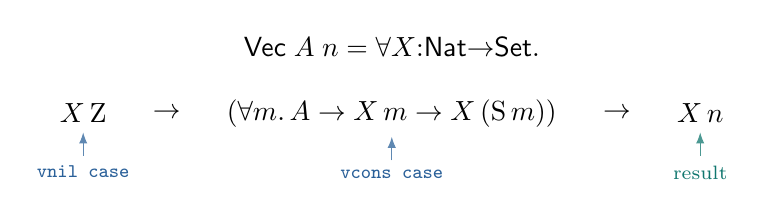
\begin{tikzpicture}[node distance=0.28cm and 0.34cm]
      \node (nil) {$X\,\mathrm{Z}$};
      \node[right=of nil] (a1) {$\to$};
      \node[right=of a1] (cons)
        {$(\forall m.\,A \to X\,m \to X\,(\mathrm{S}\,m))$};
      \node[right=of cons] (a2) {$\to$};
      \node[right=of a2] (result) {$X\,n$};
      \node[above=0.30cm of cons] (prefix)
        {$\mathsf{Vec}\;A\;n = \forall X{:}\Nat{\to}\SetS.$};

      \node[below=0.30cm of nil,font=\scriptsize\ttfamily,text=srcBlue]
        (nillabel) {vnil case};
      \node[below=0.30cm of cons,font=\scriptsize\ttfamily,text=srcBlue]
        (conslabel) {vcons case};
      \node[below=0.30cm of result,font=\scriptsize,text=tgtTeal]
        (resultlabel) {result};
      \draw[-{Latex[length=1.4mm]},srcBlue!75]
        (nillabel.north) -- (nil.south);
      \draw[-{Latex[length=1.4mm]},srcBlue!75]
        (conslabel.north) -- (cons.south);
      \draw[-{Latex[length=1.4mm]},tgtTeal!75]
        (resultlabel.north) -- (result.south);
    \end{tikzpicture}\par
  \end{sourcecard}

  \pause
  \smallskip
  \begin{columns}[T,onlytextwidth]
    \column{0.31\textwidth}
    \begin{neutralcard}{Datum $=$ eliminator}
      \small A value is what can be folded into every suitable motive $X$.
    \end{neutralcard}
    \column{0.31\textwidth}
    \begin{sourcecard}{Indexed motive}
      \small $X : \Nat \to \SetS$ lets \src{Vec}, \src{Fin}, and \src{Fmt}
      compute.
    \end{sourcecard}
    \column{0.31\textwidth}
    \begin{targetcard}{\texttt{sprintf}'s motive}
      \small $X\,Y = \mathsf{Str} \to Y$ computes the function arity.
    \end{targetcard}
  \end{columns}

  \note{%
    \textbf{[10:00 — 11:10]}\\
    There is one more CoC detail worth seeing. Our source is bare CoC, without
    native inductive declarations. The REPL's Inductive command expands to an
    indexed Böhm--Berarducci encoding. Here a vector of A at length n is defined
    by its fold: for every family X indexed by naturals, give me the empty case
    and the cons case, and I produce X n.\\
    \click The motive X depends on the index. The first argument supplies the
    \texttt{vnil} case; the second supplies \texttt{vcons}; applying the encoded
    vector to both produces $X\,n$. Vec, Fin, equality, and Fmt therefore receive
    indexed folds that compute as ordinary CoC lambda terms. For Fmt, sprintf
    chooses the motive ``a string accumulator producing Y.'' The Y is precisely
    the function type computed by the format, so the arity is represented as
    F-omega type structure after extraction. The ceiling is also precise: this
    gives indexed folds, not full dependent induction or large elimination. I
    have that distinction in the backup slides.
  }
\end{frame}

\begin{frame}{Dynamize: when data is used as a type}
  \begin{center}
  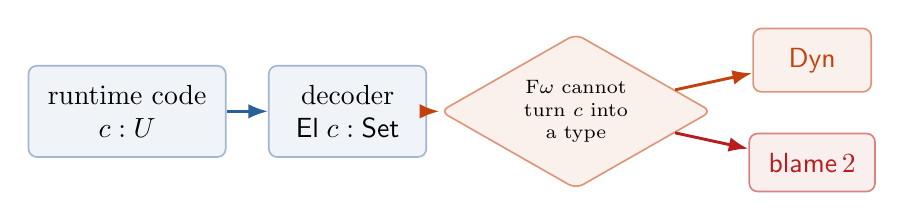
\begin{tikzpicture}
    \node[source node,minimum width=1.5cm] (code) at (0,0)
      {runtime code\\$c : U$};
    \node[source node,minimum width=2.0cm] (el) at (2.8,0)
      {decoder\\$\mathsf{El}\;c : \SetS$};
    \draw[flow arrow,srcBlue] (code) -- (el);

    \onslide<2->{%
      \node[dynamic node,diamond,aspect=1.75,inner sep=2pt,
        text width=1.7cm,font=\scriptsize]
        (gap) at (5.7,0) {\mbox{F$\omega$ cannot}\\turn $c$ into\\a type};
      \draw[flow arrow,dynOrange] (el) -- (gap);
      \node[dynamic node,minimum width=1.5cm] (dyn) at (8.7,0.65) {$\dyn$};
      \node[danger node,minimum width=1.5cm] (bl) at (8.7,-0.65) {$\blame{2}$};
      \draw[flow arrow,dynOrange] (gap) -- (dyn);
      \draw[flow arrow,blameRed] (gap) -- (bl);
    }
  \end{tikzpicture}
  \end{center}

  \onslide<2->{%
  \begin{center}\small
    The decoder is abstract in bare CoC: defining it requires large elimination.
  \end{center}}

  \onslide<3->{%
  \begin{alertblock}{The fallback is deliberately visible}
    Internal blame is reachable. It says ``this translation cannot represent
    the requested dependency'' --- a defined outcome, not undefined behavior.
  \end{alertblock}}
  \note{%
    \textbf{[11:10 — 12:25]}\\
    Dynamization is the genuinely hard residue. Imagine a universe of codes and
    a decoder El. A code is ordinary runtime data, but El turns it into a type.
    In the bare-CoC artifact this decoder is abstract, because defining it by
    large elimination is itself beyond the source calculus.\\
    \click F-omega can compute with types, but it cannot turn the runtime value
    c into a type. When a source type depends on c in this way, its translation
    uses Dyn. If that unrepresentable type-level object is demanded as a term,
    extraction inserts a reserved internal blame marker cast through Dyn.\\
    \click The result does not cover execution of every dependent program. It
    gives this unrepresentable case an explicit, typed outcome in the target
    semantics, instead of silently asserting an impossible type equality and
    allowing a host-language failure later.
  }
\end{frame}

\begin{frame}{The target's runtime contract}
  \begin{columns}[T,onlytextwidth]
    \column{0.31\textwidth}
    \begin{successcard}{\Large\faCheckCircle\quad 1}
      \large\textbf{A value}

      \smallskip
      \normalsize The computation is finished.
    \end{successcard}
    \column{0.31\textwidth}
    \onslide<2->{\begin{targetcard}{\Large\faArrowRight\quad 2}
      \large\textbf{A step}

      \smallskip
      \normalsize $e \reduces e'$ by deterministic rules.
    \end{targetcard}}
    \column{0.31\textwidth}
    \onslide<3->{\begin{dangercard}{\Large\faExclamationTriangle\quad 3}
      \large\textbf{Blame}

      \smallskip
      \normalsize $\blame{p}$ names a checked boundary.
    \end{dangercard}}
  \end{columns}

  \onslide<4->{%
  \bigskip
  \begin{successcard}{\faLock\quad Progress $+$ preservation}
    \centering A closed, well-typed term is a value, takes a step, or reports
    blame; every step preserves its type.
  \end{successcard}}
  \note{%
    \textbf{[12:25 — 13:35]}\\
    The target is System F-omega --- a language with polymorphism and functions
    over types --- extended with Dyn, checked casts, and blame. You do not need
    its grammar to understand its contract. A closed, well-typed term may
    already be a value.\\
    \click Or it can take a step, according to a deterministic operational
    semantics.\\
    \click Or it can be an explicit blame term carrying a label. A cast
    mismatch does not fall off the end of the semantics and does not invoke an
    unchecked host-language operation.\\
    \click We prove progress and preservation for the complete target. Together,
    they say that stepping preserves the type and that a closed, well-typed term
    is a value, takes a step, or reports blame. A cast mismatch therefore stays
    inside the target semantics as blame rather than becoming a host-language
    failure.
  }
\end{frame}

%% ==========================================================================
\section{Why this is hard}
%% ==========================================================================

\begin{frame}{Hard part 1: classify every binder semantically}
  \begin{center}
  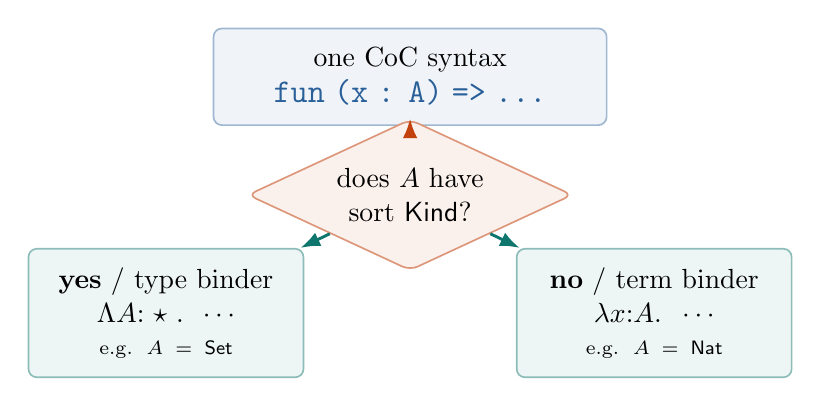
\begin{tikzpicture}
    \node[source node,text width=4.5cm] (src) at (0,1.35)
      {one CoC syntax\\[0.25ex]\large\src{\texttt{fun (x : A) => ...}}};

    \onslide<2->{%
      \node[dynamic node,diamond,aspect=2.15,text width=2.25cm,inner sep=2pt]
        (class) at (0,-0.15) {does $A$ have\\sort $\KindS$?};
      \draw[flow arrow,dynOrange] (src) -- (class);
      \node[target node,text width=3.0cm] (type) at (-3.1,-1.65)
        {\textbf{yes} / type binder\\$\Lambda A{:}\kstar.\;\cdots$\\[-0.1ex]
         \scriptsize e.g. $A = \SetS$};
      \node[target node,text width=3.0cm] (term) at (3.1,-1.65)
        {\textbf{no} / term binder\\$\lambda x{:}A.\;\cdots$\\[-0.1ex]
         \scriptsize e.g. $A = \Nat$};
      \draw[flow arrow,tgtTeal] (class) -- (type);
      \draw[flow arrow,tgtTeal] (class) -- (term);
    }
  \end{tikzpicture}
  \end{center}

  \onslide<3->{%
  \begin{center}
    \talkpill{tgtTeal}{reduction-stable classification $+$ split target namespaces}
  \end{center}}
  \note{%
    \textbf{[13:35 — 14:50]}\\
    The first implementation difficulty is the namespace mismatch we just saw.
    CoC deliberately treats
    programs and types uniformly. These two binders have the same syntactic
    form: one binds a type A and one binds a value n.\\
    \click F-omega separates those worlds. A becomes a type abstraction, while
    n becomes an ordinary function argument. The translation must also compress
    one source de Bruijn namespace into separate target type and term
    namespaces.\\
    \click We cannot make this choice by looking for a particular surface
    syntax, because an annotation may compute before revealing what it is. We
    use the semantic question ``does this have sort Kind?'' The source
    normalization and subject-reduction results are what let us prove that this
    classification does not change under computation.
  }
\end{frame}

\begin{frame}{Hard part 2: equality of types includes computation}
  \begin{center}
    \talkpill{srcBlue}{definitionally equal in CoC:\quad
      $(\lambda X{:}\SetS.\,X)\;\Nat \;\reduces\; \Nat$}
  \end{center}

  \pause
  \smallskip
  \begin{center}
  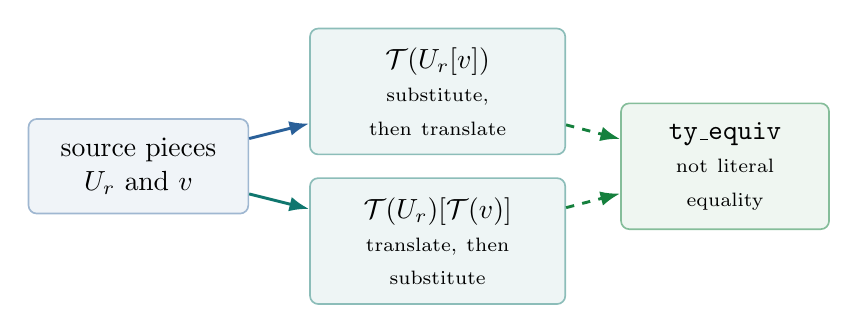
\begin{tikzpicture}
    \node[source node,text width=2.3cm] (start) at (-3.8,0)
      {source pieces\\$U_r$ and $v$};
    \node[target node,text width=2.75cm] (top) at (0,0.95)
      {$\extt(U_r[v])$\\\scriptsize substitute, then translate};
    \node[target node,text width=2.75cm] (bot) at (0,-0.95)
      {$\extt(U_r)[\extt(v)]$\\\scriptsize translate, then substitute};
    \node[success node,text width=2.15cm] (eq) at (3.65,0)
      {\texttt{ty\_equiv}\\\scriptsize not literal equality};
    \draw[flow arrow,srcBlue] (start) -- (top);
    \draw[flow arrow,tgtTeal] (start) -- (bot);
    \draw[flow arrow,okGreen,dashed] (top) -- (eq);
    \draw[flow arrow,okGreen,dashed] (bot) -- (eq);
  \end{tikzpicture}
  \end{center}

  \onslide<3->{%
  \begin{center}
    \talkpill{blameRed}{character-for-character equality is false}
    \hspace{0.4em}
    \talkpill{okGreen}{conversion absorbs the static gap}
  \end{center}}
  \note{%
    \textbf{[14:50 — 16:05]}\\
    The second difficulty is that types compute. A type-level identity function
    applied to Nat is definitionally equal to Nat even though the syntax is
    different. Every decision made by the extraction has to respect that
    equality.\\
    \click The hardest application case compares two routes: substitute a
    source type argument and then translate, or translate both pieces and
    substitute in the target. A paper proof might casually say these commute.\\
    \click They do not commute by literal equality. One route contains a target
    beta redex, and normalizing source annotations introduces another mismatch.
    The correct theorem says the two target types are equal after type-level
    computation. That discovery forced the target typing judgment to include a
    conversion rule. The exact equation is in the backup slides.
  }
\end{frame}

\begin{frame}{Hard part 3: the proof is part of the program}
  \begin{center}
  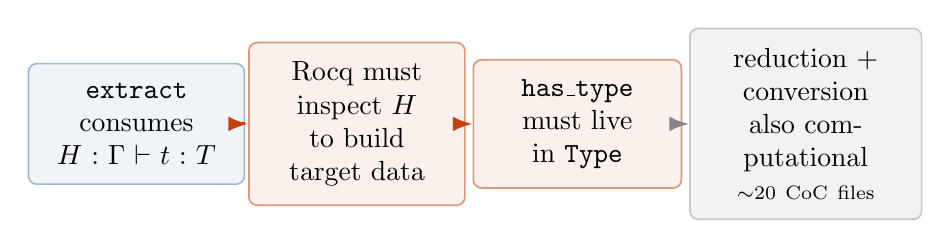
\begin{tikzpicture}
    \node[source node,text width=2.25cm] (d) at (-4.2,0.55)
      {\texttt{extract} consumes\\$H : \Gamma \vdash t : T$};
    \onslide<2->{%
      \node[dynamic node,text width=2.25cm] (elim) at (-1.4,0.55)
        {Rocq must inspect $H$\\to build target data};
      \draw[flow arrow,dynOrange] (d) -- (elim);
    }
    \onslide<3->{%
      \node[dynamic node,text width=2.15cm] (type) at (1.4,0.55)
        {\texttt{has\_type}\\must live in \texttt{Type}};
      \node[neutral node,text width=2.45cm] (infra) at (4.3,0.55)
        {reduction $+$ conversion\\also computational\\\scriptsize $\sim$20 CoC files};
      \draw[flow arrow,dynOrange] (elim) -- (type);
      \draw[flow arrow,black!48] (type) -- (infra);
    }
  \end{tikzpicture}
  \end{center}

  \onslide<4->{%
  \smallskip
  \begin{columns}[T,onlytextwidth]
    \column{0.44\textwidth}
    \begin{successcard}{\faCheckCircle\quad Derivation independence}
      \small Different typing proofs produce simulation-related extractions.
    \end{successcard}
    \column{0.52\textwidth}
    \begin{dangercard}{Mechanization changed the design}
      \small The determinism proof exposed a real overlapping reduction rule.
    \end{dangercard}
  \end{columns}}
  \note{%
    \textbf{[16:05 — 17:35]}\\
    The third difficulty is specific to making the translation an object inside
    Rocq. Extraction follows the typing derivation because that derivation tells
    it which application and binder cases it is translating.\\
    \click But Rocq separates proof-only propositions from computational data.
    It does not let a function inspect a Prop proof in order to return arbitrary
    Type data.\\
    \click So \texttt{has\_type} had to live in Type. That decision propagated
    into well-formedness, one-step and multi-step reduction, conversion,
    confluence, normalization bridges, and inference across about twenty source
    files, even though the translation function itself is small.\\
    \click Finally, typing derivations are not unique, so we prove derivation
    independence. The determinism proof also found two operational rules that
    really overlapped, so the mechanization led to a change in the target
    semantics.
  }
\end{frame}

%% ==========================================================================
\section{Evidence and scope}
%% ==========================================================================

\begin{frame}{What Rocq actually checks}
  \begin{columns}[T,onlytextwidth]
    \column{0.48\textwidth}
    \begin{sourcecard}{\faCheckCircle\quad Static guarantee}
      \small Well-typed source $\rightsquigarrow$ well-typed target.
    \end{sourcecard}
    \smallskip
    \onslide<3->{\begin{targetcard}{\faRoute\quad Source behavior}
      \small Source reduction is tracked by a deliberately \emph{syntactic} simulation.
    \end{targetcard}}

    \column{0.48\textwidth}
    \onslide<2->{\begin{successcard}{\faArrowRight\quad Dynamic guarantee}
      \small Types are preserved; execution yields a value, a step, or blame.
    \end{successcard}}
    \smallskip
    \onslide<4->{\begin{dynamiccard}{\faLock\quad Boundary guarantee}
      \small No external labels in isolation; exact characterization of Dyn-free types.
    \end{dynamiccard}}
  \end{columns}

  \onslide<5->{%
  \medskip
  \begin{center}
    \talkpill{okGreen}{fully mechanized $+$ admit-free}
    \hspace{0.45em}
    \talkpill{okGreen}{audit: \texttt{eq\_rect\_eq} only}
  \end{center}}
  \note{%
    \textbf{[17:35 — 19:05]}\\
    The checked results fall into four groups. First, the translation is type
    preserving: if Rocq accepts the source, the extracted term is accepted by
    the target at the translated type.\\
    \click Second, the target itself is safe: preservation maintains those types
    and progress gives the value-step-or-blame trichotomy.\\
    \click Third, a source reduction is tracked by the extraction. I want to be
    precise: this theorem uses a syntactic bookkeeping relation, not contextual
    or observational approximation.\\
    \click Fourth, an isolated extracted term never invents a client-owned blame
    label, and a separate theorem gives an exact syntactic characterization of
    which source types translate without Dyn.\\
    \click All of these results are machine checked, with no admitted lemmas or
    project-local axioms. The audit reports only the standard equality axiom
    shown here. The theorem names and exact statements are in the backup deck.
  }
\end{frame}

\begin{frame}[fragile]{Evidence you can poke at}
  \begin{columns}[T,onlytextwidth]
    \column{0.59\textwidth}
    \begin{beamercolorbox}[wd=\linewidth,sep=0.85em,rounded=true]{terminal card}
      \small\ttfamily
      {\color{accentOrange}Coc \textless} {\color{white}Infer}\\
      \quad fun (A : {\color{srcBlue!45!white}Set}) (x : A) => x.\\
      {\color{okGreen!65!white}Inferred: forall (A : Set), A -> A}\\[0.8ex]
      {\color{accentOrange}Coc \textless} {\color{white}Extract}\\
      \quad fun (A : {\color{srcBlue!45!white}Set}) (x : A) => x.\\
      {\color{tgtTeal!55!white}Extracted: fun (A : *) (x : A) => x}
    \end{beamercolorbox}

    \column{0.37\textwidth}
    \pause
    \begin{targetcard}{\faCubes\quad Artifact breadth}
      {\color{tgtTeal}\fontsize{23}{24}\selectfont\bfseries 18}
      \hspace{0.35em}{\small\bfseries checked batches}

      \smallskip
      \scriptsize Vectors, printf, matrices, units,\\[-0.1ex]
      AVL trees, sessions, and more.
    \end{targetcard}
    \smallskip
    \begin{dangercard}{\faExclamationTriangle\quad Stock baseline}
      {\color{blameRed}\fontsize{21}{22}\selectfont\bfseries 7/18}
      \hspace{0.35em}{\small\bfseries stock examples}

      \smallskip
      \scriptsize expose \texttt{Obj.magic} or \texttt{Obj.t}.
    \end{dangercard}
  \end{columns}

  \note{%
    \textbf{[19:05 — 20:20]}\\
    The artifact also extracts the source type checker and the mathematical
    translation to OCaml, with a small REPL around them. The first command
    infers the source type of polymorphic identity; the second prints its target
    extraction.\\
    \click The repository includes eighteen golden example batches: vectors,
    printf, dimensioned matrices, units of measure, balanced trees, session
    types, interpreters, and heterogeneous data. We also ported the same idioms
    to ordinary CIC and ran stock Rocq 9.0 extraction; seven expose unchecked
    casts or Obj.t interfaces. Even de Bruijn-to-named recovery is proved
    capture-free. To scope that accurately, the theorem covers name recovery,
    not the parser, the final string formatting, or the OCaml wrapper around the
    extracted code.
  }
\end{frame}

\begin{frame}{What this is --- and is not}
  \begin{columns}[T,onlytextwidth]
    \column{0.48\textwidth}
    \begin{neutralcard}{\faCode\quad Mathematical translation}
      \small Total and verified, but normalizes types and invokes inference:
      not a production back end.
    \end{neutralcard}
    \smallskip
    \onslide<3->{\begin{neutralcard}{\faProjectDiagram\quad Syntactic simulation}
      \small Not contextual equivalence or a full compiler-correctness theorem.
    \end{neutralcard}}

    \column{0.48\textwidth}
    \onslide<2->{\begin{dangercard}{\faExclamationTriangle\quad Reachable internal blame}
      \small A type that depends on a runtime value can deliberately fail.
    \end{dangercard}}
    \smallskip
    \onslide<4->{\begin{dynamiccard}{\faLockOpen\quad Executable boundary}
      \small No proof erasure or native inductives; opaque proof bodies are accessed.
    \end{dynamiccard}}
  \end{columns}

  \onslide<5->{%
  \smallskip
  \begin{center}
    \talkpill{tgtTeal}{boundaries today $\rightsquigarrow$ roadmap to an algorithmic compiler}
  \end{center}}
  \note{%
    \textbf{[20:20 — 21:35]}\\
    The result has four important limits. First, the translation is a total
    mathematical function on typing derivations, but it normalizes types and
    calls a decision procedure. It is not an efficient production back end,
    even though the REPL lets us run examples.\\
    \click Second, internal blame is intentionally reachable. It marks a source
    type that depends on runtime data in a way F-omega cannot represent.\\
    \click Third, simulation is syntactic. We do not yet prove that arbitrary
    typed program contexts observe equivalent behavior; that needs a new typed
    logical relation.\\
    \click Fourth, the current translation does not erase proof terms, the bare
    CoC source models inductive families rather than adding native CIC
    inductives, and Rocq extraction of the executable accesses opaque
    computational proof bodies.\\
    \click These limitations do not weaken the stated theorems. They say exactly
    what stage of the design space this artifact establishes.
  }
\end{frame}

%% ==========================================================================
\section{Takeaways}
%% ==========================================================================

\begin{frame}{Takeaways}
  \begin{columns}[T,onlytextwidth]
    \column{0.48\textwidth}
    \begin{dangercard}{1 / The handoff is a boundary}
      Verified source code still needs a safe target interface.
    \end{dangercard}
    \smallskip
    \onslide<3->{\begin{dynamiccard}{3 / Make residue explicit}
      Dependencies beyond F$\omega$ cross a $\dyn$-and-blame boundary.
    \end{dynamiccard}}

    \column{0.48\textwidth}
    \onslide<2->{\begin{targetcard}{2 / Preserve the static skeleton}
      F$\omega$ keeps \texttt{sprintf}'s arity and makes index erasure explicit.
    \end{targetcard}}
    \smallskip
    \onslide<4->{\begin{successcard}{4 / Check the whole story}
      Rocq verifies target safety and extraction metatheory, admit-free.
    \end{successcard}}
  \end{columns}

  \onslide<5->{%
  \medskip
  \begin{center}
    \small Preserve what F$\omega$ can express and represent the remainder with
    \textcolor{blameRed}{blame},\\[-0.1ex]
    rather than hiding the boundary behind \texttt{Obj.magic}.
  \end{center}}
  \note{%
    \textbf{[21:35 — 23:00]}\\
    I will close with four claims. First, verification does not end when a source
    term is accepted. If extracted code must compose with ordinary clients, the
    exported target type is part of the safety story.\\
    \click Second, we do not need to erase all the way down to a weak ML
    interface. F-omega preserves type abstraction, type application, and
    higher-kinded structure; that is enough to make the printf mistake a static
    error again.\\
    \click Third, when full dependency really exceeds the target, we make the
    residue explicit with Dyn and internal blame. It may fail, but it fails
    inside the semantics instead of corrupting the runtime.\\
    \click Fourth, Rocq checks both the target calculus and the translation, with
    the assumptions audited and no admits.\\
    \click The design rule is to preserve what F-omega can express, represent the
    remainder with Dyn and blame, and never hide that boundary with Obj.magic.
  }
\end{frame}

\begin{frame}[standout]
  Thank you!

  \medskip
  {\normalsize
    \src{CoC} $\longrightarrow$ \tgt{System F$\omega$}
    $+$ $\dyn$ $+$ \textcolor{blameRed}{blame}}

  \medskip
  {\small
  \texttt{dune exec tests/top.exe} --- try the REPL\\
  Full Rocq development, examples, paper, and Q\&A backup slides in the artifact}
  \note{%
    \textbf{[23:00+] — Q\&A.}\\
    Thank you! I'm happy to take questions. I have backup slides with the full
    target grammar, blame labels, the compatibility rules, the exact conversion
    lemma, theorem names, and the inductive encoding. I can also run the REPL if
    that would be useful.
  }
\end{frame}

%% ==========================================================================
%% Q&A BACKUP SLIDES — deliberately unnumbered
%% ==========================================================================

\appendix
\section{Backup}

\begin{frame}[noframenumbering]{Backup: why F$\omega$ rather than ML?}
  \begin{columns}[c,onlytextwidth]
    \column{0.44\textwidth}
    \begin{sourcecard}{Computed return type in CIC}
      \small\ttfamily
      eval : expr t ->\\
      \quad match t with\\
      \qquad NatCode => Nat\\
      \qquad BoolCode => Bool
    \end{sourcecard}

    \column{0.08\textwidth}
    \centering{\color{accentOrange}\Large\faArrowRight}

    \column{0.44\textwidth}
    \begin{targetcard}{Church codes, one kind up}
      \centering\small kind $\kstar\karr\kstar\karr\kstar$\\[0.5ex]
      $\mathsf{eval} : \forall t.\;\mathsf{expr}\;t \to
        t\;\mathsf{CNat}\;\mathsf{CBool}$
    \end{targetcard}
  \end{columns}

  \medskip
  \begin{columns}[T,onlytextwidth]
    \column{0.31\textwidth}
    \begin{successcard}{Our extraction}
      \small No $\dyn$, casts, or blame.
    \end{successcard}
    \column{0.31\textwidth}
    \begin{dangercard}{Stock extraction}
      \small One of the heaviest \texttt{Obj.magic} users.
    \end{dangercard}
    \column{0.31\textwidth}
    \begin{dynamiccard}{The ceiling}
      \small Term-code computation requires large elimination.
    \end{dynamiccard}
  \end{columns}
  \note{Backup answer for ``what does F$\omega$ buy?'' The key is that a
    type-level code becomes an ordinary higher-kinded type function.}
\end{frame}

\begin{frame}[noframenumbering]{Backup: target syntax}
  \begin{columns}[T,onlytextwidth]
    \column{0.27\textwidth}
    \begin{targetcard}{Kinds}
      \centering
      $K ::= \kstar$\\[-0.2ex]
      $\mid\ K \karr K$
    \end{targetcard}
    \column{0.69\textwidth}
    \begin{targetcard}{Types}
      \centering\scriptsize
      $A,B ::= \alpha \mid A \to B \mid \forall\alpha{:}K.\,A$\\[-0.2ex]
      $\mid\ \Lambda\alpha{:}K.\,A \mid A\,B \mid \dyn$
    \end{targetcard}
  \end{columns}
  \smallskip
  \begin{neutralcard}{Terms}
    \centering\scriptsize
    \begin{align*}
      e ::= {}&x \mid \lambda x{:}A.\,e \mid e\,e
        \mid \Lambda\alpha{:}K.\,e \mid e[A]\\[-0.35ex]
        &\mid \castt{e}{A}{B}{p} \mid \gnd{e}{G} \mid \isgnd{e}{G}
        \mid \blame{p} \mid \nub{\alpha}{K}{A}{e}
    \end{align*}
  \end{neutralcard}

  \vspace{-0.4em}
  \begin{center}
    \talkpill{dynOrange}{$\dyn : \kstar$ only}
    \hspace{0.5em}
    \talkpill{tgtTeal}{neutral ground tags $N ::= \alpha \mid N\,A$}
  \end{center}
  \note{Backup grammar. The $\nu$ binder implements scoped type sealing for
    polymorphic instantiation.}
\end{frame}

\begin{frame}[noframenumbering]{Backup: reading a blame label}
  \begin{columns}[T,onlytextwidth]
    \column{0.37\textwidth}
    \begin{dangercard}{Anatomy of $\blame{42+}$}
      \begin{center}
        {\color{blameRed}\fontsize{30}{31}\selectfont\bfseries 42+}
      \end{center}
      \small
      \textbf{id 42}\quad which boundary broke\\[0.5ex]
      \textbf{polarity +}\quad blame the value\\
      \hspace*{4.3em}$-$ would blame its context
    \end{dangercard}

    \column{0.59\textwidth}
    \begin{neutralcard}{Reserved identifiers}
      \small
      \talkpill{blameRed}{0}\quad sealed type escapes $\nu$ scope through $\dyn$\\[0.65ex]
      \talkpill{blameRed}{1}\quad $\mathsf{is\_gnd}$ peeks at a sealed value\\[0.65ex]
      \talkpill{blameRed}{2}\quad source type has no F$\omega$ representation\\[0.65ex]
      \talkpill{tgtTeal}{$\ge 3$}\quad client-established external boundary
    \end{neutralcard}
  \end{columns}

  \smallskip
  \begin{center}
    \talkpill{tgtTeal}{no external labels in isolation}
    \hspace{0.4em}
    \talkpill{blameRed}{internal labels remain reachable}
  \end{center}
  \note{The external-label theorem covers extracted terms in isolation. Internal
    labels are deliberately reachable.}
\end{frame}

\begin{frame}[noframenumbering]{Backup: executable compatibility}
  Every $\mathsf{compat}(A,B)$ constructor selects an executable rule:

  \medskip
  \begin{columns}[T,onlytextwidth]
    \column{0.31\textwidth}
    \begin{targetcard}{Static shapes}
      \small
      \texttt{compat\_refl} $\to$ \textbf{ID}\\[0.6ex]
      \texttt{compat\_arrow} $\to$ \textbf{WRAP}
    \end{targetcard}
    \column{0.31\textwidth}
    \begin{targetcard}{Polymorphism}
      \small
      \texttt{compat\_all}\\
      generalize / instantiate\\[0.4ex]
      $\to$ \textbf{$\forall$-steps}
    \end{targetcard}
    \column{0.31\textwidth}
    \begin{dynamiccard}{The $\dyn$ boundary}
      \small
      to/from $\dyn$\\[0.4ex]
      $\to$ \textbf{GROUND}\\
      \textbf{COLLAPSE / CONFLICT}
    \end{dynamiccard}
  \end{columns}

  \smallskip
  \begin{center}
    \talkpill{okGreen}{no stuck casts: \texttt{progress} via \texttt{compat\_dec}}
    \hspace{0.35em}
    \talkpill{tgtTeal}{$\mathsf{coerce}$ is total}
  \end{center}
  \smallskip
  \begin{center}\small
    Caveat: compatibility is syntactic, not closed under definitional equality.
  \end{center}
  \note{Backup operational detail. Non-identity clients must normalize
    annotations before selecting compatibility.}
\end{frame}

\begin{frame}[noframenumbering]{Backup: target metatheory}
  \begin{columns}[T,onlytextwidth]
    \column{0.31\textwidth}
    \begin{successcard}{Determinism}
      \scriptsize\mech{step\_deterministic}
    \end{successcard}
    \smallskip
    \begin{successcard}{Preservation}
      \scriptsize\mech{preservation}\\
      \mech{preservation\_star}
    \end{successcard}
    \column{0.31\textwidth}
    \begin{targetcard}{Type confluence}
      \scriptsize\mech{ty\_star\_confluent}\\
      \mech{ty\_equiv\_church\_rosser}
    \end{targetcard}
    \smallskip
    \begin{targetcard}{Regularity}
      \scriptsize
      \mech{typing\_annotations}\\[-0.2ex]
      \mech{\_regular}
    \end{targetcard}
    \column{0.31\textwidth}
    \begin{successcard}{Progress}
      \scriptsize\mech{progress}\\[0.35ex]
      value / step / blame
    \end{successcard}
    \smallskip
    \begin{dangercard}{Not strongly normalizing}
      \scriptsize
      \mech{typing\_does\_not\_imply}\\[-0.2ex]
      \mech{\_strong\_normalization}
    \end{dangercard}
  \end{columns}

  \medskip
  \begin{center}
    \talkpill{srcBlue}{source normalization defines $\mathsf{nf}$}
    \hspace{0.4em}
    \talkpill{blameRed}{target safety $\ne$ target termination}
  \end{center}
  \note{Safety does not imply termination. Source CoC normalization is the
    separate fact used to define source normal forms during extraction.}
\end{frame}

\begin{frame}[noframenumbering]{Backup: the three translation maps}
  \begin{columns}[T,onlytextwidth]
    \column{0.48\textwidth}
    \begin{sourcecard}{Kinds}
      \small $\SetS \to \Nat \to \SetS$
      $\rightsquigarrow$ $\kstar \karr \kstar$; term domains drop.
    \end{sourcecard}
    \smallskip
    \begin{targetcard}{Terms}
      \small $\ext$ recurses on the typing derivation and branches using
      $\islarge$.
    \end{targetcard}
    \column{0.48\textwidth}
    \begin{dynamiccard}{Types}
      \small Normalize first; sorts, term variables, and term-headed applications
      become $\dyn$.
    \end{dynamiccard}
    \smallskip
    \begin{neutralcard}{Contexts}
      \small Compress one source namespace into target type and term namespaces.
    \end{neutralcard}
  \end{columns}

  \smallskip
  \begin{targetcard}{\faLock\quad Conversion invariant}
    \centering\scriptsize Every classification uses reduction-stable $\islarge$;
    type extraction normalizes before translation.
  \end{targetcard}
  \note{Backup translation definition. The implementation lives in
    \texttt{Extraction/translation.v}.}
\end{frame}

\begin{frame}[noframenumbering]{Backup: the exact hard application case}
  A large source application emits a bare target type application:

  \medskip
  \begin{columns}[c,onlytextwidth]
    \column{0.40\textwidth}
    \begin{targetcard}{Natural target type}
      \centering\small
      $\extt(V{:}\Gamma,U_r)[\extt(\Gamma,v)/0]$
    \end{targetcard}
    \column{0.14\textwidth}
    \centering
    \talkpill{blameRed}{$\ne$ syntax}\\[0.7ex]
    \talkpill{okGreen}{$\equiv$}
    \column{0.40\textwidth}
    \begin{targetcard}{Expected target type}
      \centering\small
      $\extt(\Gamma,U_r[v])$
    \end{targetcard}
  \end{columns}

  \medskip
  \begin{center}
    \talkpill{blameRed}{target $\beta$-redex}
    \hspace{0.4em}
    \talkpill{blameRed}{normal-form annotation drift}
  \end{center}

  \medskip
  \begin{successcard}{The proved statement}
    \scriptsize\mech{extract\_typ\_tsubst\_coc\_equiv} gives target
    $\mathsf{ty\_equiv}$; \mech{typing\_conv} absorbs the gap with no runtime cast.
  \end{successcard}
  \note{This was the final large-application well-typedness obligation. Literal
    equality is false; target definitional equality is exactly the right notion.}
\end{frame}

\begin{frame}[noframenumbering]{Backup: headline extraction theorems}
  \begin{columns}[T,onlytextwidth]
    \column{0.48\textwidth}
    \begin{sourcecard}{1 / Well typed}
      \scriptsize\mech{extract\_well\_typed}
    \end{sourcecard}
    \smallskip
    \begin{targetcard}{2 / Reduction simulation}
      \scriptsize\mech{extract\_reduces\_once}, \mech{extract\_reduces}
    \end{targetcard}
    \smallskip
    \begin{successcard}{3 / Derivation independence}
      \scriptsize\mech{extract\_deriv\_indep}
    \end{successcard}

    \column{0.48\textwidth}
    \begin{dynamiccard}{4 / External-label safety}
      \scriptsize\mech{extraction\_blame\_free}
    \end{dynamiccard}
    \smallskip
    \begin{targetcard}{5 / Syntactic instantiation}
      \scriptsize\mech{extraction\_instantiation\_sim}
    \end{targetcard}
    \smallskip
    \begin{successcard}{6 / Exact Dyn-freedom}
      \scriptsize\mech{extract\_typ\_dyn\_free\_iff}
    \end{successcard}
  \end{columns}

  \smallskip
  \begin{center}
    \talkpill{okGreen}{audit: \texttt{eq\_rect\_eq} only \quad$\bullet$\quad
      \texttt{extract\_typ\_wf\_sort} axiom-free}
  \end{center}
  \note{The audited theorem set depends only on \texttt{eq\_rect\_eq};
    \texttt{extract\_typ\_wf\_sort} is axiom-free.}
\end{frame}

\begin{frame}[noframenumbering]{Backup: the encoding's ceiling}
  \begin{columns}[T,onlytextwidth]
    \column{0.46\textwidth}
    \begin{successcard}{\faCheckCircle\quad What the encoding gives}
      \begin{itemize}\small
        \item motives parameterized by indices
        \item genuine computation by indexed folds
        \item Vec, Fin, Eq, and Fmt recursors
      \end{itemize}
    \end{successcard}

    \column{0.50\textwidth}
    \begin{dangercard}{\faTimesCircle\quad What it cannot give}
      \begin{itemize}\small
        \item motive depending on the eliminated value
        \item dependent induction / large elimination
        \item one-step inversion without axioms
      \end{itemize}
    \end{dangercard}
  \end{columns}

  \medskip
  \begin{neutralcard}{Other encodings do not erase the ceiling}
    \small Scott/Parigot need recursive types; Mendler reaches the same induction
    boundary; self types go further but extend beyond CoC.
  \end{neutralcard}
  \note{Backup answer about native inductives and large elimination. Extending
    the source from CoC to CIC is future work.}
\end{frame}

\end{document}
